% Explanation of the experiments and results (included by explanation.tex).
\section{The experiments and how to read the results}
\subsection{What was measured, and how}
\begin{itemize}
\item \textbf{Time.} One ``run'' is one complete shortest-path computation from one source (start vertex) to \emph{all} vertices, over the whole graph and all its edges. It includes resetting the labels but not loading the graph. The option \code{--sources N} is the number of different start vertices, not a number of edges: 20 on the five road networks, 10 on the SNAP graphs, 3 on generated graphs. Every algorithm is run from the same sources; for each source the run is repeated (9 times on road networks, 3 on SNAP graphs, 5 on generated graphs) and the median is kept. Results differ little between start vertices on the same graph. To compare two algorithms the ratio of their times is taken \emph{for each source separately}, and the geometric mean of these ratios is reported. A ratio of 4 means ``four times slower than Dijkstra''.
\item \textbf{Counts.} A second executable built from the same source code (\code{bin/sssp\_count}) increments a counter at every comparison of two labels or keys (including those inside heaps, search trees and the selection routine), at every addition $\dhat[u]+w_{uv}$, and at every edge scan. All counts are divided by the number of edges $m$, so ``1.0 scans per arc'' means every edge was looked at once on average.
\item \textbf{Baseline.} ``Dijkstra'' always means the binary-heap version with lazy deletion (\code{DijkstraLazy}); ``Dijkstra (DecreaseKey)'' is the indexed-heap variant.
\item \textbf{Settings.} Unless a table says otherwise, the new algorithms run on the graph as it is (no degree reduction), with the parameters their papers prescribe and with the three repairs of Section~\ref{sec:fixes}.
\end{itemize}

\subsection{The data}
The five road networks are Oldenburg (OL, 6\,105 vertices), San Joaquin County (TG, 18\,263), California (CAL, 21\,048), San Francisco (SF, 174\,956) and North America (NA, 175\,813). Each line of an edge file is one road segment with its length. Segments are used in both directions (see Section~\ref{sec:verified} for why), so the graphs have between 14\,070 and 446\,002 directed edges. They are very sparse (2.0 to 2.6 edges per vertex) and ``thin'': when Dijkstra runs on them its heap never holds more than \RoadPeakMax\% of the vertices at once.

Six larger real graphs from the SNAP collection were added after looking at \code{bzantium/bmssp-python}, which benchmarks on them (Section~\ref{sec:snapex}). They are downloaded by \code{sh scripts/fetch\_data.sh snap}.

In addition, four families of generated graphs were added to see what happens as graphs grow to millions of vertices: random graphs, grids, ``preferential attachment'' graphs with a few very high-degree vertices, and ``hub'' graphs designed so that Dijkstra starts with all $n$ vertices in its heap.

\subsection{Road networks: time (paper Table V; this chart is only in the guide)}
\begin{center}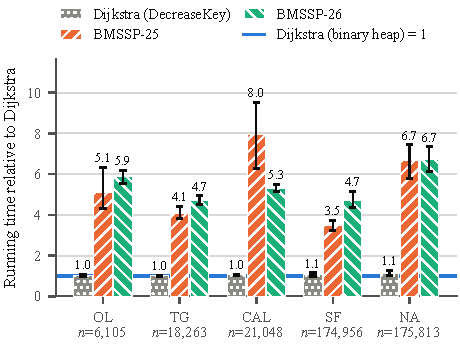
\includegraphics[width=0.62\textwidth]{real_ratio}\end{center}
Each group of bars is one network. The blue line at height 1 is Dijkstra. A bar of height 5 means that algorithm needed five times as long. The thin whiskers show the best and worst source. Reading: \bmA{} is \RealRatioMinTwoFive--\RealRatioMaxTwoFive{} times slower and \bmB{} is \RealRatioMinTwoSix--\RealRatioMaxTwoSix{} times slower than Dijkstra; the two Dijkstra variants are practically equal. \bmB{} beats \bmA{} on only \RealTwoSixFasterWord{} of the five networks.

\subsection{Road networks: counts (paper Table VI and Fig.~1)}
\begin{center}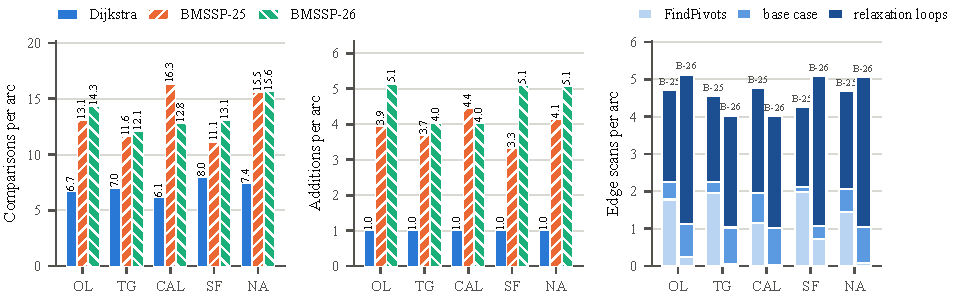
\includegraphics[width=\textwidth]{real_counts}\end{center}
Left and middle panel (in the paper these numbers are Table VI): comparisons and additions per edge. Dijkstra makes 6--8 comparisons and exactly 1 addition per edge. The new algorithms make 11--16 comparisons and 3--5 additions. So on road networks they are slower \emph{already in the abstract cost model}, before any hardware effects.

Right panel (this is Fig.~1 of the paper): how often each edge is scanned, and in which part of the algorithm. Dijkstra: once. \bmA{} (bars marked B-25): 4--5 times, of which more than one whole pass happens inside FindPivots (light blue). \bmB{} (B-26): 4--5 times as well, but almost none of it in FindPivots. This is the clearest picture of what the 2026 paper changed: pivot finding became cheap. The dark part (relaxation loops) is larger for 2026 because every recursion level relaxes every edge once and the 2026 parameters give one more level on three of the five networks.

\emph{Cost per operation.} If an algorithm needs 4.5 times the time but only 2 times the operations, each of its operations costs about 2.3 times as much. This number is \PerOpMinTwoFive--\PerOpMaxTwoFive{} for \bmA{} and \PerOpMinTwoSix--\PerOpMaxTwoSix{} for \bmB. It reflects things the abstract model ignores: bigger labels, bookkeeping, and memory accesses that the processor cannot predict.

\subsection{Validation table (paper Table IV)}
Rows: the algorithm as printed in its paper and with the repairs. Columns: number of runs; runs with a wrong distance (always 0); runs in which a stale key was seen; runs in which a vertex was reported complete twice; runs in which the base-case boundary invariant was violated. Reading: the stale keys occur in both algorithms; without the deletion they cause duplicate completions; with the repairs the duplicate and boundary columns are zero.

On the real road networks these effects are rare (duplicates are at most \DupPctMaxTwoFive\% of the vertices) and make no measurable difference to the running time; they matter for whether the published proofs apply, not for speed.

\subsection{Degree reduction (paper Table VII)}
The proofs assume a graph in which every vertex has very few edges. Transforming the road networks into that form makes them \ReduceNGrowMin--\ReduceNGrowMax{} times larger, and every algorithm becomes several times slower on the transformed graph. Conclusion: the transformation is needed for the proofs, but in practice one should not apply it. (Castro et al.\ found the same for the 2025 algorithm.)

\subsection{Parameter sweep (paper Fig.~2)}
\begin{center}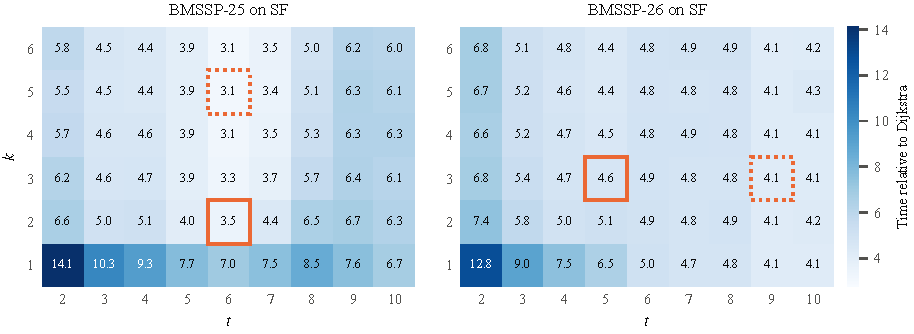
\includegraphics[width=\textwidth]{params_heatmap}\end{center}
Each cell is one choice of $(k,t)$ on the San Francisco network; the number is the time relative to Dijkstra (smaller and lighter is better). The solid orange box is the choice prescribed by the paper, the dotted box the best one found. Reading: $k=1$ (bottom row) is bad, which shows that reducing the frontier really is necessary; the prescribed parameters are reasonable; tuning gains \ParSFTwoFiveGain\% (2025) and \ParSFTwoSixGain\% (2026) on SF and \ParNATwoFiveGain\% and \ParNATwoSixGain\% on NA; but even the best cell is about \ParSFTwoFiveBest{} times slower than Dijkstra.

\subsection{Growing graphs: time (paper Fig.~3)}
\begin{center}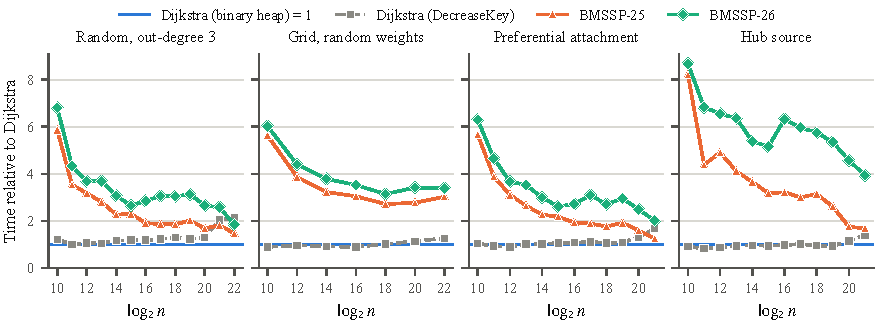
\includegraphics[width=\textwidth]{scaling_ratio}\end{center}
Four families of generated graphs, sizes from about a thousand to about four million vertices (the horizontal axis is $\log_2 n$, so each step doubles the size). Vertical axis: time relative to Dijkstra (blue line at 1). Reading:
\begin{itemize}
\item \emph{Random graphs and preferential-attachment graphs:} the new algorithms catch up steadily as graphs grow. \bmA{} goes from \ScaleRandTwoFiveFirst{} times slower at $2^{10}$ to \ScaleRandTwoFiveLast{} times slower at $2^{22}$ on random graphs, and to \ScaleBaTwoFiveLast{} on the largest preferential-attachment graph. They never get below the blue line.
\item \emph{Grids:} no catching up beyond a certain point; both stay between \GridLateMin{} and \GridLateMax{} times slower.
\item \emph{Hub graphs:} \bmA{} reaches \ScaleHubTwoFiveLast, \bmB{} stays at \ScaleHubTwoSixLast.
\item \bmB{} (green) is above \bmA{} (orange) in every panel: it was slower on all \SynthPoints{} generated graphs.
\item The zig-zags come from rounding: $k$, $t$ and the number of levels are whole numbers and jump at certain sizes.
\end{itemize}

\subsection{Growing graphs: counts (paper Fig.~4)}
\begin{center}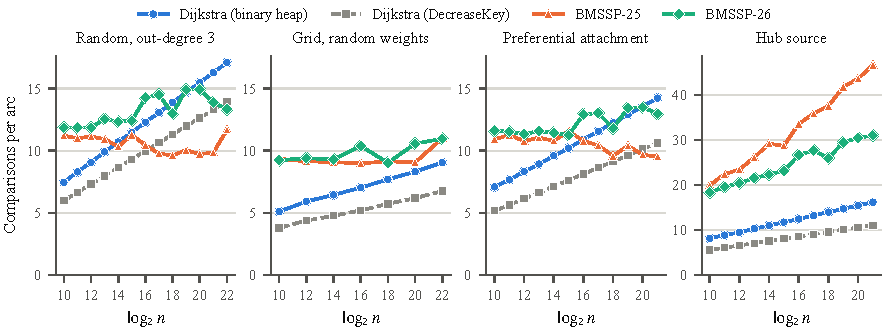
\includegraphics[width=\textwidth]{scaling_cmp}\end{center}
This is the most interesting figure: comparisons per edge as the graphs grow. (The additions per edge are in \code{figure\_data.txt} and are quoted in the text.)
\begin{itemize}
\item On \emph{random} and \emph{preferential-attachment} graphs the blue Dijkstra line climbs steadily (about \SlopeRandDij{} more comparisons per edge every time the graph doubles: that is the $\log n$ of the sorting barrier), while the orange \bmA{} line stays flat at about 10. The lines cross: from $n=2^{\CrossCmpRandTwoFiveDij}$ (random) and $2^{\CrossCmpBaTwoFiveDij}$ (preferential attachment) on, \bmA{} needs fewer comparisons than Dijkstra, and from $2^{\CrossOpsRandTwoFiveDij}$ and $2^{\CrossOpsBaTwoFiveDij}$ on also fewer comparisons plus additions. \bmB{} gets below Dijkstra's comparison count at about a million vertices. \textbf{So the theoretical advantage is real and already visible at ordinary sizes, if one counts operations.}
\item It is still slower on the clock. At $2^{20}$ random vertices \bmA{} performs \OpsRandTwentyTwoFive{} operations per edge against Dijkstra's \OpsRandTwentyDij, yet needs \TimeRandTwentyTwoFive{} times the time. The abstract model does not charge for looking at every edge 3--5 times, for wider labels or for the bookkeeping of the block structures.
\item On \emph{grids} (and road networks) there is no crossing. Reason: Dijkstra's heap stays tiny there (on the largest grid it never holds more than \PeakGrid\% of the vertices; on random graphs \PeakRand\%). With a small heap Dijkstra has almost no sorting work that could be saved.
\item On \emph{hub} graphs (note the different vertical scale) the new algorithms do far more comparisons, although the frontier is as wide as possible. Reason: the source has an edge to every other vertex, which breaks the ``small degree'' assumption. All these edges arrive in the data structure at once and get fully sorted. Paper Table VIII checks this explanation: after the degree-reduction transformation the same graph satisfies the assumption, and then \bmB{} needs less than half of Dijkstra's comparisons (\HubRedCmpTwoSix{} against \HubRedCmpDij{} per original edge). But the transformed graph is eight times larger, so everything is slower than plain Dijkstra on the original graph (\HubCmpDij{} comparisons per edge).
\end{itemize}
\textbf{Take-away on graph structure.} Two properties decide how the new algorithms compare with Dijkstra: how wide Dijkstra's frontier gets (wide is good for the new algorithms), and whether some vertex has a huge degree (bad for them unless the graph is transformed, which is costly).


\subsection{The graphs from bzantium's repository (paper Table IX)}\label{sec:snapex}
Six graphs from the SNAP collection, the same ones bzantium's README uses: two web graphs (Stanford, Google), three road networks (Pennsylvania, Texas, California) and the Pokec social network, with 0.3 to 2 million vertices and up to 30.6 million edges. They have no weights, so each is run twice: with all weights 1 (what bzantium does) and with random weights.

Reading of the table: Dijkstra is the fastest on all \SnapInstances{} instances. \bmA{} is \SnapRatioMinTwoFive--\SnapRatioMaxTwoFive{} times slower and \bmB{} \SnapRatioMinTwoSix--\SnapRatioMaxTwoSix{} times slower. The advantage that bzantium's table shows for its ``V2'' solver therefore does not exist for the real algorithm on the very same graphs.

The comparison counts again follow the frontier rule. The three SNAP road networks have narrow frontiers (at most \SnapRoadPeakMax\% of the vertices) and the new algorithms need more comparisons than Dijkstra (\SnapCmpRoadMinTwoFive--\SnapCmpRoadMaxTwoFive{} times for \bmA). The web and social graphs have wide frontiers (\SnapOtherPeakMin--\SnapOtherPeakMax\%), and there \bmA{} needs between \SnapCmpOtherMinTwoFive{} and \SnapCmpOtherMaxTwoFive{} times Dijkstra's comparisons: fewer than Dijkstra on \SnapFewerCmpTwoFive{} of the \SnapInstances{} instances. So the pattern found on generated graphs also shows on real ones.

\subsection{Density and weight range (paper Section VI-I; this chart is only in the guide)}
\begin{center}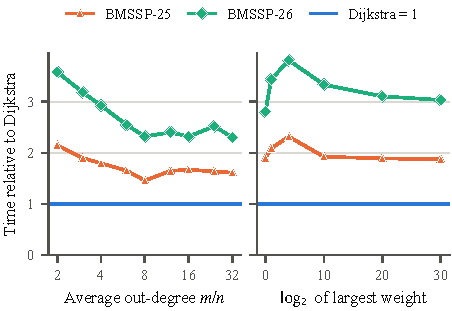
\includegraphics[width=0.62\textwidth]{sweeps}\end{center}
Left: random graphs with more and more edges per vertex. The new algorithms get relatively better up to about 8 edges per vertex and then level off (ratios \DensMinTwoFive--\DensMaxTwoFive{} for 2025, \DensMinTwoSix--\DensMaxTwoSix{} for 2026). Right: the size of the weights hardly matters, not even in the extreme case where all weights are 1 and many comparisons are decided by the tie-breaking rule.

\subsection{Memory (paper Section VI-J)}
On the 4-million-vertex random graph the whole program needed \MemDij~MB with Dijkstra, \MemTwoFive~MB with \bmA{} and \MemTwoSix~MB with \bmB. The extra memory is mainly the per-level lookup tables.
